
\chapter{Benchmarks and analysis framework}
\label{sec:org17c0cef}

In this chapter we describe the benchmarks that will be mapped to the Surface-17 chip and the simulation framework develop for the study of the mapping metrics.

\section{Benchmarks}
\label{sec:orga02804b}
In order to analyze the different metrics to assess the quality of a mapping algorithm, we selected a set of quantum algorithms available in the literature.

I built a list of quantum algorithms coming from different sources.
The sources we chose are RevLib \cite{Wille_2008}, ScaffCC \cite{JavadiAbhari_2015}, some benchmarks from Zulehner's et al. work \cite{zulehner17:effic_method_mappin_quant_circuit} and QLib \cite{Lin_2014} because of the variety of algorithms and because they are already decomposed in the Clifford+T set.
Note that the language used to describe the algorithm varies from source to source.
Although, they all use a  a QASM-based language, there are small syntax differences.
As we will explain in the next section, we will use our own programming languages -- OpenQL and cQASM -- and compiler.
Therefore we had to translate all the selected algorithms from their QASM versions to the OpenQL notation.
I developed a parser in order to do that.

I also profiled each benchmark including: the number of qubits of the algorithm, the number of gates, the functionality of the algorithm and different graphs, showing the percentage of the operations types or the degree of parallelism of the algorithm.
Most of the benchmarks are classical algorithms adapted to quantum circuits.
They are deterministic and then the result is always the same if there are no errors.
%This means that their results are always binary.
This is because  at the end of the circuit, before measuring the qubits, qubits are in either ground or excited state, but never superposition.


The benchmarks were also classified depending on their functionality.
This is an important step because algorithms that do similar calculations are used to have common gates distribution.
From all the benchmarks we have, we can distinct six different classes.

\begin{itemize}
\item Quantum Gates: Circuits that are a decomposition of a Quantum Gate
\item Search Algorithms
\item Worst Cases: Circuits that were really difficult to generate for RevLib
\begin{itemize}
\item HWB: is the simplest function with exponential Ordered Binary Decision Diagrams (OBDD) size.
\end{itemize}
\item Encoding Functions: Classical codification functions
\item Arithmetic Functions: Functions that perform an arithmetic operation
\item Miscellaneous: Mix of different kind of algorithms
\end{itemize}

We came up with a list of 84 different algorithms -- 697 benchmarks taking into account the different versions of the same functionality -- that can be found in the \href{https://github.com/QE-Lab/qbench}{qbench Github repo}, as well as the previous information in much more detail.
These algorithms cannot only be used for the mapping problem but also for other activities in our group.

\subsection{Benchmark selection}
\label{sec:org80c681f}

In order to have a small, but representative, set of benchmarks to map, we selected just some of them.
This requirement comes by the fact that simulations are long and computationally exhaustive.
In order to do that, we studied the different benchmark profiles looking for most illustrative cases.
The criteria used for selecting the algorithms used in this work are: 
i) the number of qubits of the algorithm. It should be less than 17 as we will use the Surface-17 chip; ii) the number of gates.
We select benchmarks with a number of gates as spread as possible; iii) different functionality.
We try to have the less number of the same algorithm versions as possible.
We only take the same algorithm versions for cases in which the number of qubits and the number of gates show an interesting combination.
For example, two similar algorithms which number of qubits or number of gates are very distinct as the first three selected benchmarks in Tab. \ref{tab:map_selected_benchs}.

Once we had our requirements we could start the analysis and the selection afterwards.
In Tab. \ref{tab:map_selected_benchs} we show the final benchmark selection.
\begin{table}[htbp]
\caption{\label{tab:org0f8ca31}
Restriction summary of the benchmark selection}
\centering
\begin{tabular}{|l|}
\hline
\\
Criteria:\\
\\
- \# qubits < 17\\
- \# gates as spread as possible and in the case of repeated benchmark the minimum number of gates\\
- The less number of the same algorithm versions/classes as possible\\
- The benchmarks that are repeated and have an interesting combination of No. qubits/No. gates are  preferred\\
\\
\hline
\end{tabular}
\end{table}
43 benchmarks (with qubits numbers from 3 to 17 qubits) selected after applying the previous Restrictions to the analysis of the benchmarks described in the next section (see Table \ref{tab:map_selected_benchs}).
After simulating the algorithms, few of them returned errors (segmentation fault) and some others .

\section{Analysis framework}
\label{sec:orgc0c805b}
In this section we introduce the framework used to map the quantum algorithms and analyze the quantum metrics.
It is based on two steps: \textbf{compilation} and \textbf{simulation}.
With this purpose we connect two tools, OpenQL and quantumsim \textcolor{red}{Please, add a refernce to qauntumsim and OpenQL}, and we build a whole framework over them.

\subsection{Compiler (OpenQL)}
\label{sec:orgeebd0c8}
OpenQL is a framework for high-level quantum programming developed by our group to describe quantum algorithms and compile them.
The framework can be found as a library in either C++ or Python and, therefore, the circuits are described over one of these programming languages. It can target real quantum chips as well as different quantum computer simulators such are QX simulator or quantumsim \textcolor{red}{add references here to both simulators}. 

One of the passes of the compiler is the \textbf{mapper} algorithm developed by our group. It performs the initial placement, schedule the operations and route the qubits taking into account the quantum chip constraints that are described in a JSON file.
It is also able to load different compiler configurations like the kind of scheduler, router or initial placement.
We will use OpenQL to describe the selected benchmarks and compile them for the SC-17 chip.
In Fig. \ref{code:openql_gray_code} we show an example of OpenQL code using Python that describes the Gray encoder quantum circuit (Fig. \ref{fig:circuit_example}).
More insights can be found in the \href{https://github.com/QE-Lab/OpenQL}{github repository}.

\begin{figure}
\centering
\begin{minipage}{\textwidth}

\begin{minted}[frame=lines,fontsize=\scriptsize,linenos,breaklines,breakanywhere]{python}

from openql import openql as ql

def circuit(config_file, scheduler='ASAP', uniform_sched= 'no', mapper='base', initial_placement='no', output_dir_name='test_output', optimize='no', measurement=True, log_level='LOG_WARNING'):
    curdir = os.path.dirname(__file__)
    output_dir = os.path.join(curdir, output_dir_name)
    ql.set_option('output_dir', output_dir)
    ql.set_option('optimize', optimize)
    ql.set_option('scheduler', scheduler)
    ql.set_option('scheduler_uniform', uniform_sched)
    ql.set_option('mapper', mapper)
    ql.set_option('initialplace', initial_placement)
    ql.set_option('log_level', log_level)

    config_fn = os.path.join(curdir, config_file)

    platform  = ql.Platform('starmon', config_fn)
    sweep_points = [1,2]
    num_circuits = 1
    num_qubits = 6
    p = ql.Program('graycode6', platform, num_qubits)
    p.set_sweep_points(sweep_points, num_circuits)
    k = ql.Kernel('graycode6', platform, num_qubits)
    k.gate('cnot',[1,0])
    k.gate('cnot',[2,1])
    k.gate('cnot',[3,2])
    k.gate('cnot',[4,3])
    k.gate('cnot',[5,4])

    if measurement:
	for q in range(num_qubits):
	    k.gate('measure', [q])

    p.add_kernel(k)
    p.compile()

\end{minted}

\caption{OpenQL description in python code describing the Gray code algorithm.}
\label{code:openql_gray_code}
\end{minipage}
\end{figure}

\subsection{quantumsim}
\label{sec:org96b0d71}

Quantumsim \cite{O_Brien_2017} is a simulator for superconducting systems and designed to study the SC-17 chip.
Its error model has been induced from the chip's behaviour after several experiments.
Therefore, quantumsim's error model is much more complete for the superconducting case than other general simulators.
It is based in the decoherence time and the observed gate error rates.
Although the detail in its error model makes each simulation computationally harder.
As a matter of fact, quantumsim is able to boost its calculations with a Graphics Processing Unit (GPU).
Quantumsim can be found as a \textbf{python library} in its \href{https://github.com/quantumsim/quantumsim}{github repository} with instructions to install it and an overview of how to use it.

\subsection{Analysis Framework}
\label{sec:org60b7659}
In order to study the metrics, we developed a simulation framework.
This framework was developed in order to be a tool extensively used by our group.
For this reason it was thought as a modular system.
The framework maps a quantum algorithm to a given device, using OpenQL.
Then it simulates it with quantumsim.
Later on, the framework will execute an analysis of the simulation results.
The analysis is based on the fidelity, probability of success and quantum volume calculations besides the depth, number of added SWAPs and the total number of operations extracted from the different circuit descriptions.
Finally, all the data is stored in a database with the aim to do an exercise of data analysis to study the mapping metrics.
The framework flow can be followed in the Fig. \ref{fig:general_error_framework}.
Note that, although we choose quantumsim to run our experiments, we could have introduced any other simulator due to the modular nature of the framework.



\begin{sidewaysfigure}[ht]

\begin{center}
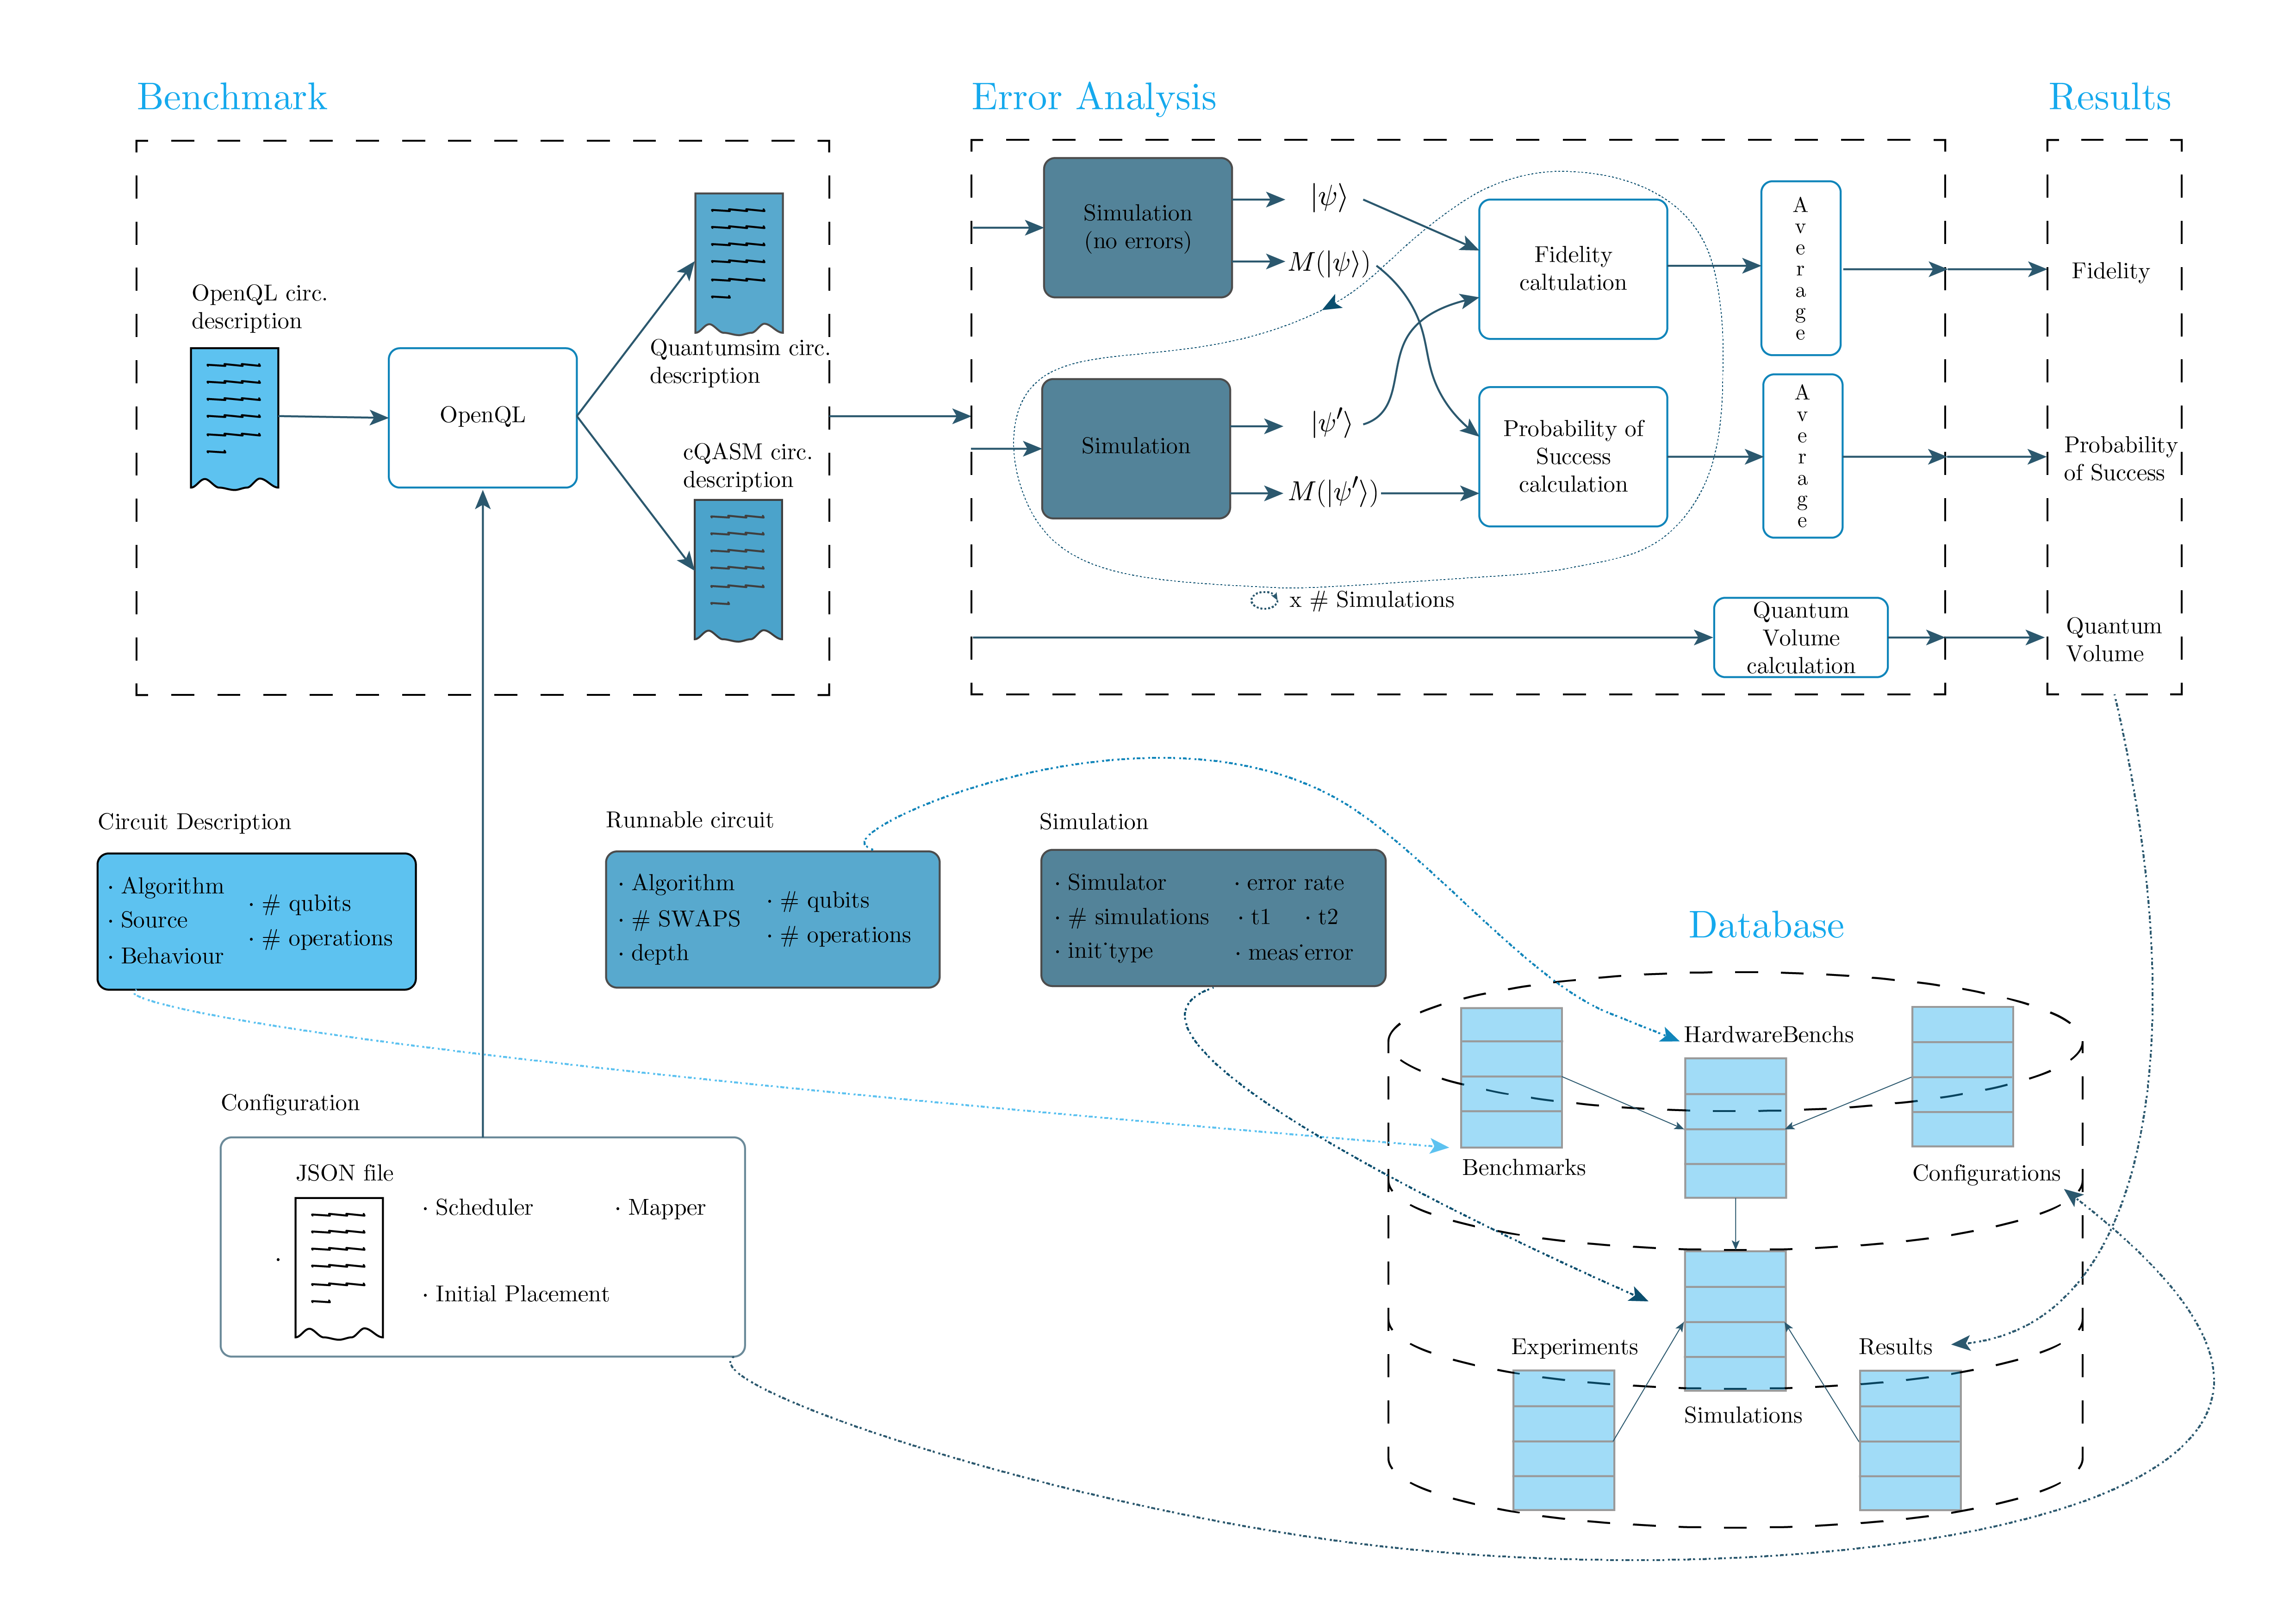
\includegraphics[width=.9\linewidth]{figures/error_framework_diagram.png}
\end{center}


    \caption{Analysis Framework}
    \label{fig:general_error_framework}
\end{sidewaysfigure}

\begin{enumerate}
\item Benchmark mapping
\label{sec:orge67926f}

First, the framework compiles the benchmarks described in OpenQL depending on the \textbf{configuration} introduced.
The configuration options are the mapper characteristics (scheduler, initial placement and router) and the JSON file describing the quantum device for which the algorithm should be mapped.
OpenQL exports the mapped version of the circuit in a language understandable by a simulator, in either quantumsim or cQASM \cite{khammassi18} code.
From all the circuits descriptions -- before and after being mapped --, the framework extracts the algorithm name, the number of qubits used and the number of operations.
Also, from the circuits before mapping it will extract the source and the functionality and from the ones mapped the depth and the number of SWAPs added.
All this information will be stored in the database.

\item Mapping simulation
\label{sec:org033fd05}

After being mapped, the simulator will load the mapped circuit and the simulation characteristics.
The mapped algorithm will be simulated first without errors, in order to know what is the correct result or the result we should expect from this circuit.
We store both, the resultant quantum state \(\psi\) and its ideal measurement \(M(\psi)\).
Note that, as soon as our benchmarks are all deterministic (see the \hyperref[sec:orga02804b]{Benchmarks} section) the quantum state and the measurement will be the same.
After saving the correct result, the framework proceeds to simulate \(N\) times the benchmark.
The results affected by the errors will be used to calculate the fidelity -- between the quantum state \(\psi'\) and the expected one \(\psi\) -- as well as the probability of success -- between the measurement \(M(\psi')\) and the expected one \(M(\psi)\).
The final value for fidelity and probability of success will be calculated averaging all the fidelities and probabilities of success calculated per simulation.
At the same time the quantum volume will be calculated with the depth and the number of qubits from the qubits mapped.
Finally these results and the simulations parameters will be stored in the database.

\item Database
\label{sec:orgb5f5bb4}

The database is conformed by six different tables.
The \emph{Benchmarks} table will store the information from the circuits before being mapped: the algorithm name, its source and functionality, the number of qubits used and the number of operations.
The \emph{Configurations} table will save the device configuration and the mapper characteristics.
\emph{HardwareBenchs} will store the name, the number of qubits and operations from the mapped algorithms as well as the SWAPs added and the circuit depth.
\emph{Simulations} will save the simulator options as the simulator used, the number of simulations, the error rate, the decoherence times and the measurement error.
The \emph{Results} table stores all the results from the simulations and the \emph{Experiments} table saves data about the moment when the framework was used in order to identify the different experiments done.
\end{enumerate}
